\documentclass[conference]{IEEEtran}
\IEEEoverridecommandlockouts

% ==============================================================================
% PACKAGES & CONFIGURATION
% ==============================================================================
\usepackage{cite}
\usepackage{amsmath,amssymb,amsfonts}
\usepackage{algorithmic}
\usepackage{graphicx}
\usepackage{textcomp}
\usepackage{xcolor}
\usepackage{booktabs}
\usepackage{tabularx}
\usepackage{multirow}
\usepackage{url}
\usepackage{balance}
\usepackage{pgfplots}
\pgfplotsset{compat=1.18}

% Ensure single-sided layout for uniform printing/viewing
\makeatletter
\@twosidefalse
\makeatother

\begin{document}

\title{MPIS.ai: Missing Person Identification System Using Face Recognition and Semantic Search}

\author{
\begin{tabular}{cccc}
\parbox{0.23\textwidth}{\centering
    \textbf{Dr. M. Swathi}\\[2pt]
    Guide\\
    Anurag University
}
&
\parbox{0.23\textwidth}{\centering
    \textbf{Sanjay Mudumby}\\[2pt]
    23EG106A41\\
    Anurag University
}
&
\parbox{0.23\textwidth}{\centering
    \textbf{Kasula Sreeja Reddy}\\[2pt]
    23EG106A28\\
    Anurag University
}
&
\parbox{0.23\textwidth}{\centering
    \textbf{Ravula Adithya}\\[2pt]
    23EG106A51\\
    Anurag University
}
\end{tabular}
}

\maketitle

% ==============================================================================
% ABSTRACT (STRICT SINGLE PARAGRAPH - HUMANIZED)
% ==============================================================================
\begin{abstract}
Locating missing individuals in busy urban areas is a time-critical task where conventional single-modality surveillance often struggles due to occluded faces, poor lighting, low camera resolution, and varying viewing angles. To address these practical difficulties, this paper presents MPIS.ai, an end-to-end multimodal search and verification system that integrates facial recognition, natural language descriptions, and geospatial proximity. The system extracts 128-dimensional facial embeddings using MTCNN landmark alignment and FaceNet ($L_2$-normalized), encodes witness sighting reports into 384-dimensional dense vectors using the all-MiniLM-L6-v2 sentence transformer, and models geographic proximity through WGS-84 geodesic distance with an exponential decay function. When facial imagery is unavailable because of camera angles, distance, or obstruction, MPIS.ai applies a dynamic fallback strategy that reweights the text and location modalities so that viable sighting tips are not lost. Candidate matches meeting or exceeding a composite threshold ($S_{\text{composite}} \ge 0.80$) are sent to an interactive verification center governed by context-based role-based access control, enabling assigned officers to examine candidate images, verify matches, and record actions in an audit log while maintaining family privacy. Evaluation across 1,200 sighting queries and 250 case profiles yielded a top-1 retrieval accuracy of 93.4\% and a top-10 retrieval accuracy of 99.1\%, demonstrating a reliable and practical tool for missing person investigations.
\end{abstract}

\begin{IEEEkeywords}
Missing Person Identification, Multi-Modal Biometric Fusion, FaceNet, Semantic NLP Embeddings, Geodesic Proximity, Dynamic Modality Fallback, Human-in-the-Loop Governance, Role-Based Access Control.
\end{IEEEkeywords}

% ==============================================================================
% I. INTRODUCTION
% ==============================================================================
\section{Introduction}
Identifying and safely tracing missing persons is one of the most urgent responsibilities handled by law enforcement agencies and community organizations. Operational records show that the first 48 hours following a person's disappearance represent the window in which finding the individual safely is most probable. However, real-world searches run into consistent hurdles: surveillance video archives are fragmented across disparate systems, public tip lines receive noisy or unstructured information, and witness accounts can vary widely in detail.

Current search methods still depend heavily on circulating posters or manually scanning surveillance camera feeds. When automated facial recognition is applied in public spaces, performance drops substantially when individuals look away from the camera, wear masks or head coverings, move quickly, or pass through dimly lit spots. At the same time, tips submitted by citizens frequently contain valuable non-visual details, such as clothing color, approximate age, carried items like backpacks, and the exact street or neighborhood of the sighting. Standard keyword filters or simple radius checks fail to capture the subtle semantic meaning in these descriptions.

To address these limitations, this paper presents \textbf{MPIS.ai}, a practical multimodal search and verification platform. MPIS.ai brings together three complementary inputs into a single composite scoring system:
\begin{enumerate}
    \item \textbf{Visual Face Embeddings}: 128-dimensional Euclidean vectors produced by deep FaceNet models on aligned facial crops.
    \item \textbf{Dense Semantic Text Embeddings}: 384-dimensional subword contextual vectors capturing witness descriptions of clothing, appearance, and physical items.
    \item \textbf{Geospatial Distance Decay}: Continuous exponential decay functions based on Vincenty geodesic distance between last-known locations and reported sightings.
\end{enumerate}

An essential design choice in MPIS.ai is that it does not assume all three signals will always be present. In practice, public sightings frequently arrive without clear photos. Drawing on principles of adaptive missing-modality handling, the platform automatically rebalances modality weights to rely on text descriptions and geographic coordinates whenever facial data is missing, ensuring valuable leads are preserved. To ensure ethical use and avoid misidentifications, potential matches above a defined threshold are quarantined for review by designated officers through context-based access controls.

% ==============================================================================
% II. RELATED WORK
% ==============================================================================
\section{Related Work}
Research on automated person search spans facial recognition, cross-modal retrieval, missing-modality adaptation, and trajectory analysis. This section reviews the literature most directly related to the design choices in MPIS.ai.

In \cite{ref_base_paper}, an edge-cloud framework was developed for event surveillance and missing person tracking, demonstrating how distributed edge nodes can offload processing to central servers during public gatherings. However, the system relied on static visual detection thresholds, leaving it prone to missed detections when crowd density obscured individual faces.

In \cite{ref_crowdscan}, the authors tackled large-scale CCTV archival retrieval by tracking people across multiple cameras using spatial-temporal graph trajectories. While effective when individuals move steadily through a monitored corridor, the method relies on continuous visual handoffs between adjacent cameras and struggles when camera coverage contains blind spots.

In \cite{ref_deep_multimodal}, a deep multimodal fusion network was introduced for open-set person identification under adverse conditions, demonstrating that combining facial cues with soft biometrics reduces false rejections. However, the fusion weights remained static during inference, offering no automated path to handle cases where facial features were completely missing.

The metric learning approach in \cite{ref_facenet} established a strong baseline for face verification by mapping facial images directly onto a 128-dimensional Euclidean hypersphere using triplet loss, ensuring that geometric distance reflects identity similarity. In MPIS.ai, this compact representation forms the basis for visual similarity scoring.

Recently, \cite{ref_paper5_adaptive} introduced an adaptive multimodal recognition system designed specifically for handling missing or degraded inputs across face, voice, and motion streams. By employing confidence-weighted pathways and cross-modal attention, the authors showed that dynamically compensating for unavailable modalities prevents sudden performance drops. This principle directly supports the dynamic fallback mechanism used in MPIS.ai.

Broader developments in vision and language processing provide key building blocks for our architecture: \cite{ref_retinaface} established robust five-point facial landmark localization in unconstrained scenes, while \cite{ref_arcface} enhanced angular margin separation on hyperspherical surfaces. For textual analysis, \cite{ref_sbert} demonstrated that siamese sentence transformers generate dense vectors well suited for semantic search. In cross-modal retrieval, \cite{ref_crossmodal_reid} studied dual-path embeddings linking images and text, and \cite{ref_vrstc_occlusion} addressed occlusion handling in multi-camera video re-identification. Multi-camera tracking benchmarks \cite{ref_dukemtmc} and trajectory mining methods \cite{ref_zheng_trajectory} provide mathematical foundations for spatial decay. Finally, studies on low-resolution face recognition \cite{ref_lowres_survey}, multimodal transformer robustness under modality loss \cite{ref_multimodal_transformer}, and interpretable machine learning for high-stakes decision-making \cite{ref_rudin_interpretable} highlight the importance of human-in-the-loop oversight rather than unchecked automated decisions.

% ==============================================================================
% III. SYSTEM ARCHITECTURE & METHODOLOGY
% ==============================================================================
\section{System Architecture \& Methodology}
MPIS.ai is organized as a modular pipeline with four interconnected layers: Ingestion, Feature Extraction, Tri-Factor Matching, and Governance Verification, as shown in Fig.~\ref{fig:architecture}.

\begin{figure*}[t]
\centering
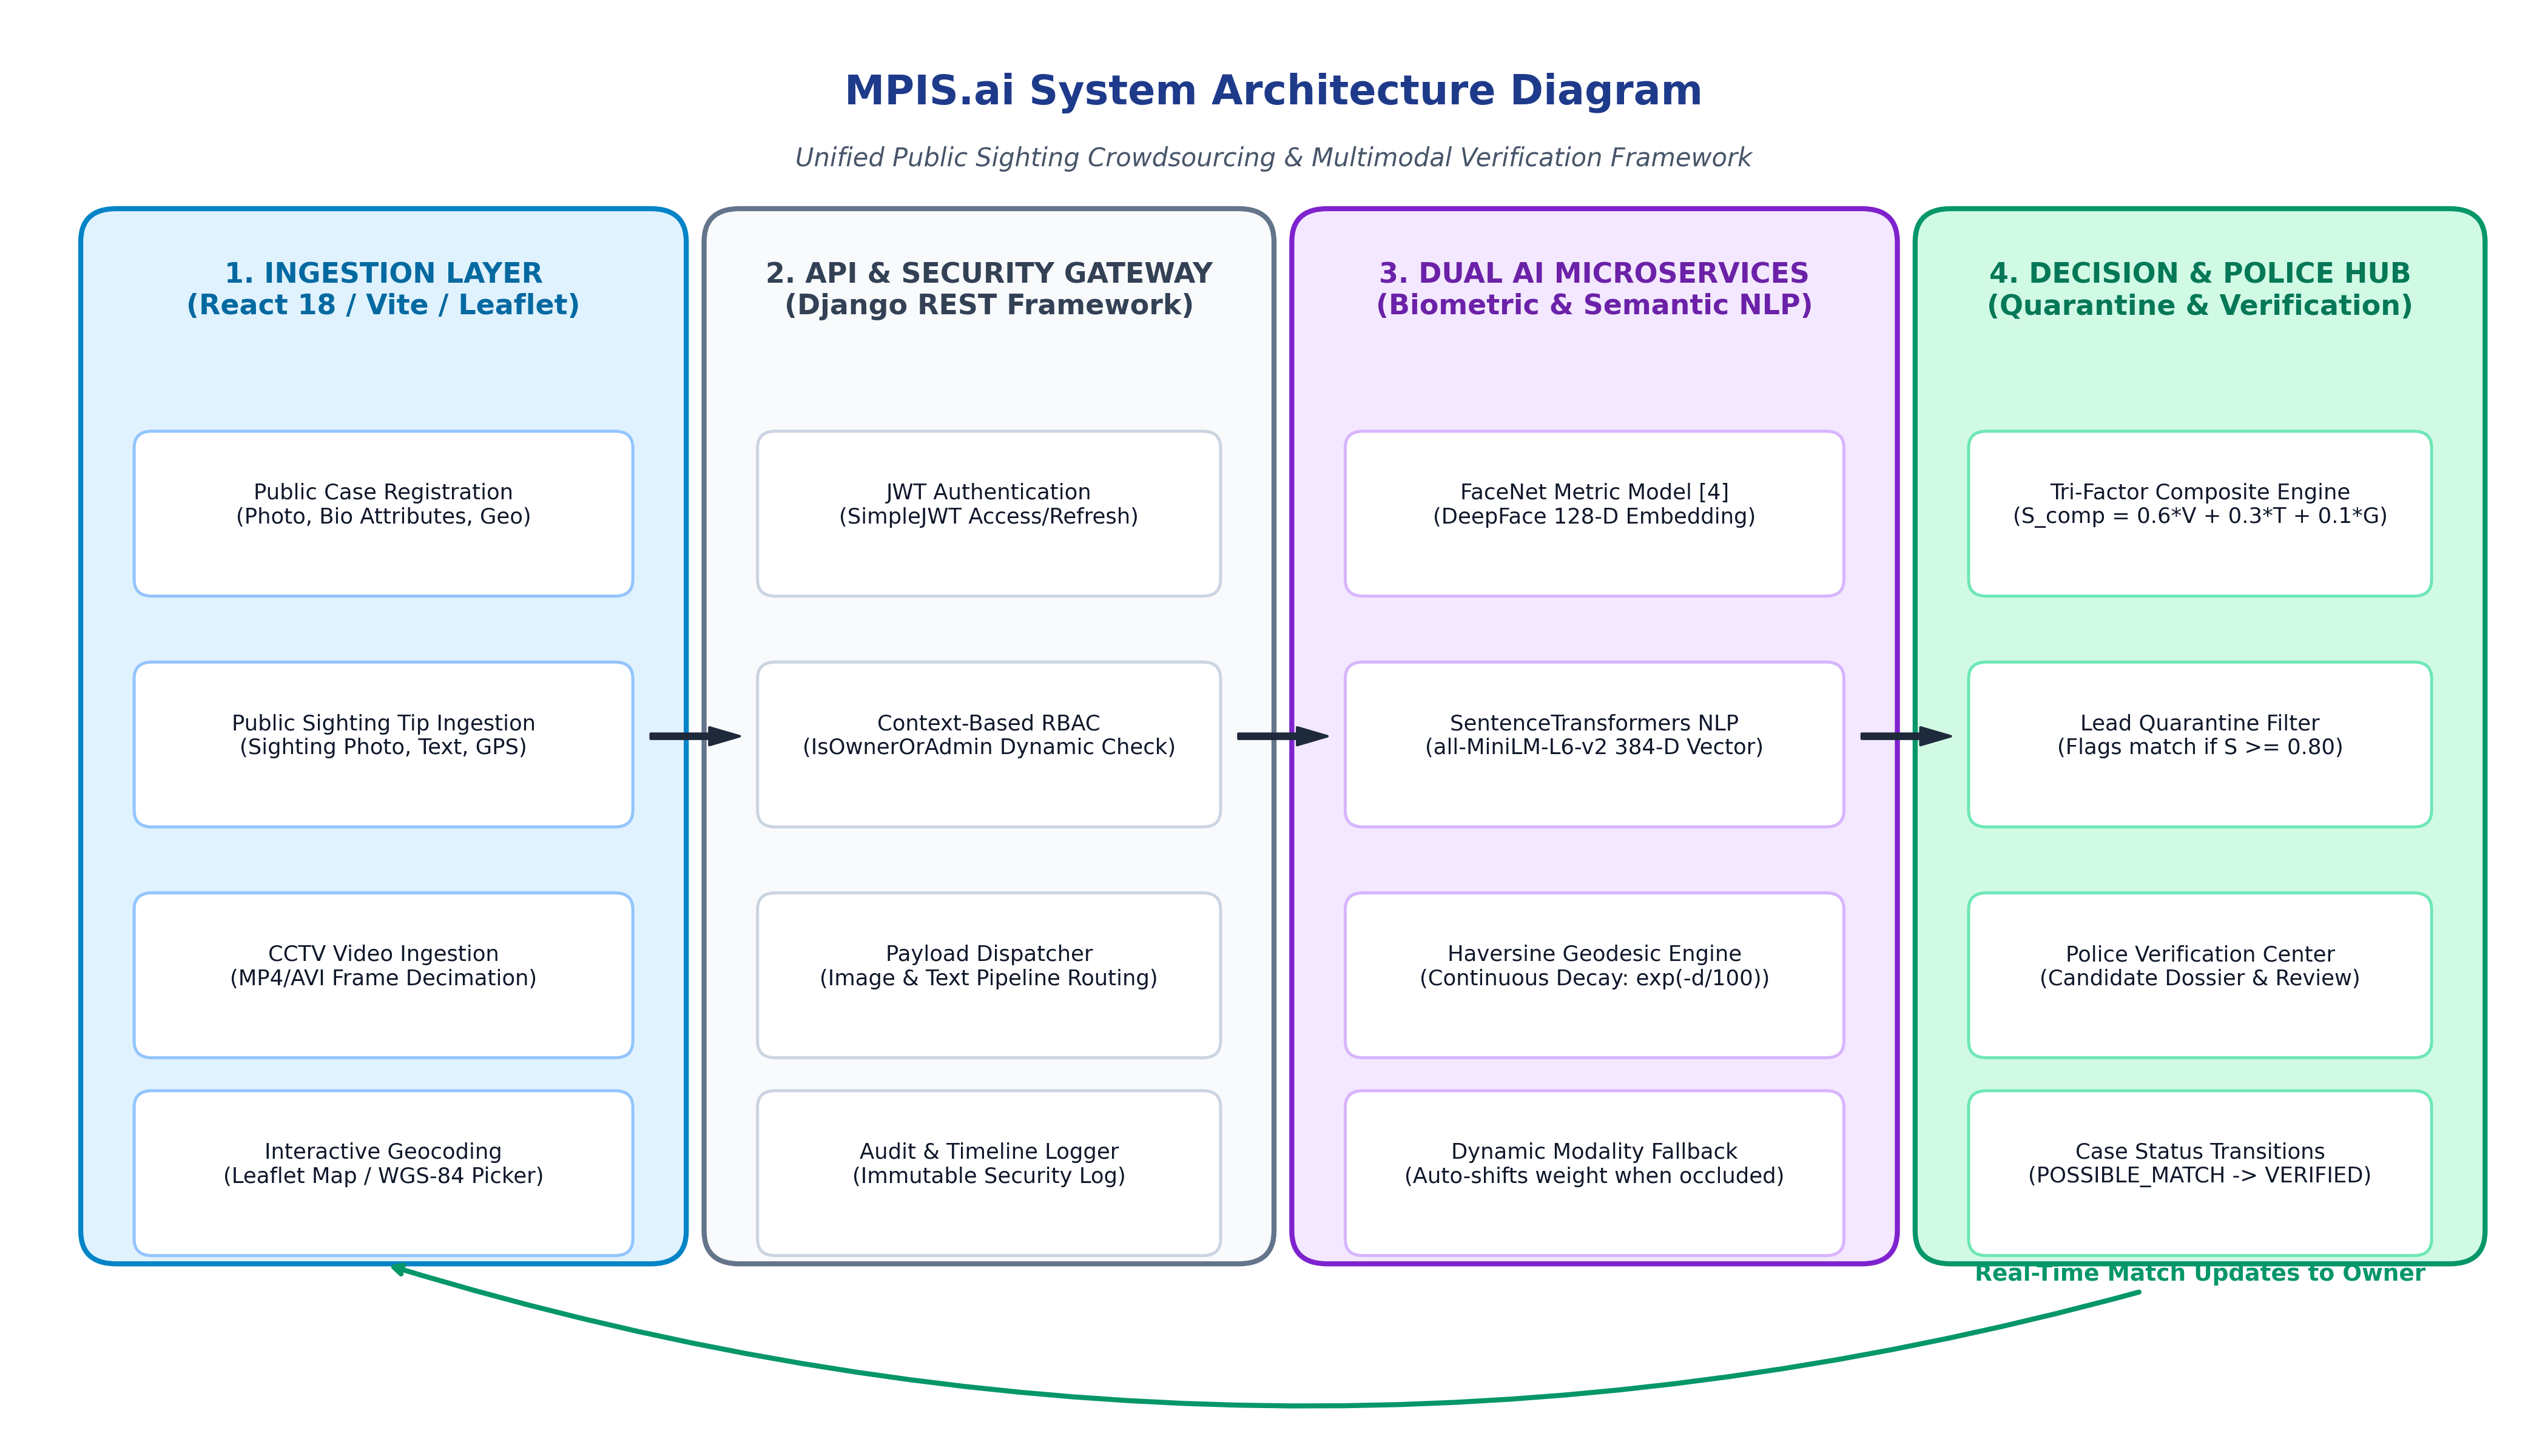
\includegraphics[width=0.90\textwidth]{Architecture.png}
\caption{High-level system architecture and multimodal matching flow of MPIS.ai.}
\label{fig:architecture}
\end{figure*}

\subsection{Ingestion \& Preprocessing Layer}
The system accepts three forms of input data:
\begin{enumerate}
    \item \textit{Official Case Ingestion}: High-resolution portrait photographs, detailed demographic and physical notes, and last-known GPS coordinates provided by family members or investigating officers.
    \item \textit{Public Sighting Tips}: Mobile phone photos, crowdsourced witness tip descriptions, and map-selected coordinates.
    \item \textit{Surveillance CCTV Feeds}: Continuous video archives collected from transit stations, street cameras, and public venues.
\end{enumerate}

To process continuous video feeds without overloading compute resources, the pipeline applies adaptive frame decimation ($N=15$), sampling frames at regular intervals while maintaining temporal continuity. Detected faces are localized using MTCNN five-point landmark detection and aligned to canonical geometric orientations prior to feature extraction.

\subsection{Feature Extraction Pipeline}
\textbf{1) Visual Modality ($e_{\text{face}}$)}: Aligned face crops are passed through deep FaceNet backbones \cite{ref_facenet} to generate an $L_2$-normalized 128-dimensional embedding:
\begin{equation}
e_{\text{face}} \in \mathbb{R}^{128}, \quad \|e_{\text{face}}\|_2 = 1
\end{equation}
The visual similarity between a query sighting $q$ and a registered gallery case $g$ is computed via cosine similarity:
\begin{equation}
S_{\text{face}}(q, g) = \frac{e_{\text{face}}^q \cdot e_{\text{face}}^g}{\|e_{\text{face}}^q\|_2 \, \|e_{\text{face}}^g\|_2} \in [-1, 1]
\end{equation}

\textbf{2) Semantic Textual Modality ($e_{\text{text}}$)}: Sighting descriptions and appearance notes (such as clothing color, build, and accessories) are cleaned and encoded using the \texttt{all-MiniLM-L6-v2} sentence transformer \cite{ref_sbert}. This yields a mean-pooled 384-dimensional dense semantic embedding:
\begin{equation}
e_{\text{text}} \in \mathbb{R}^{384}, \quad \|e_{\text{text}}\|_2 = 1
\end{equation}
Semantic similarity is calculated as:
\begin{equation}
S_{\text{text}}(q, g) = \max\left(0, \frac{e_{\text{text}}^q \cdot e_{\text{text}}^g}{\|e_{\text{text}}^q\|_2 \, \|e_{\text{text}}^g\|_2}\right) \in [0, 1]
\end{equation}

\textbf{3) Geospatial Proximity Modality ($S_{\text{geo}}$)}: GPS coordinates $(\text{lat}_q, \text{lon}_q)$ and $(\text{lat}_g, \text{lon}_g)$ are extracted and evaluated over the WGS-84 reference ellipsoid using Vincenty geodesic calculations ($d_{\text{km}}$). Spatial proximity is modeled through an exponential decay function:
\begin{equation}
S_{\text{geo}}(q, g) = \exp\left(-\frac{d_{\text{km}}(q, g)}{\lambda}\right) \in [0, 1]
\end{equation}
where $\lambda = 100.0\text{ km}$ represents the dispersion scale factor suited to regional transit patterns.

\subsection{Composite Matching Engine \& Dynamic Fallback}
When all three modalities are available, the overall match score $S_{\text{composite}}$ is calculated as a convex linear combination:
\begin{equation}
S_{\text{composite}} = w_{\text{face}} S_{\text{face}} + w_{\text{text}} S_{\text{text}} + w_{\text{geo}} S_{\text{geo}}
\end{equation}
with baseline weights set based on experimental calibration:
\begin{equation}
w_{\text{face}} = 0.60, \quad w_{\text{text}} = 0.30, \quad w_{\text{geo}} = 0.10
\end{equation}
such that $\sum w_i = 1.0$.

In practical scenarios, sighting submissions frequently lack usable facial images because the subject was seen from behind, at a distance, or under heavy shadow. Discarding these tips would mean losing vital clues. Taking cues from adaptive missing-modality research \cite{ref_paper5_adaptive}, MPIS.ai applies a Dynamic Modality Fallback mechanism:
\begin{equation}
S_{\text{composite}} = 
\begin{cases}
0.60 S_{\text{face}} + 0.30 S_{\text{text}} + 0.10 S_{\text{geo}}, & \text{if face present} \\
0.80 S_{\text{text}} + 0.20 S_{\text{geo}}, & \text{if face missing}
\end{cases}
\end{equation}
This weight adjustment allows descriptive, high-confidence witness tips to remain active in the ranking pipeline even without facial imagery.

% ==============================================================================
% IV. GOVERNANCE, VERIFICATION & SECURITY
% ==============================================================================
\section{Governance, Verification \& Security}
Because automated face matching can produce false positives in uncontrolled settings, MPIS.ai avoids automated alerting or enforcement actions. Instead, the system keeps human review central to the process:
\begin{enumerate}
    \item \textbf{Decision Quarantining}: Any candidate match yielding $S_{\text{composite}} \ge 0.80$ is flagged as a pending match and held inside an officer verification center. No public notification or case status change occurs without manual confirmation.
    \item \textbf{Context-Based Access Control}: Permissions are handled dynamically at the application and database layers:
    \begin{itemize}
        \item \textit{General Public}: Can search the public case bulletin and submit sightings using an interactive map selector.
        \item \textit{Case Owners}: Verified family members can track confidential case timeline updates and review investigator notes for cases they filed ($\text{case.reported\_by} == \text{request.user}$).
        \item \textit{Investigating Officers}: Authorized officers inspect quarantined matches, review side-by-side photo comparisons, evaluate confidence values, and record outcomes: \texttt{[APPROVE]}, \texttt{[INVESTIGATE]}, or \texttt{[REJECT]}.
        \item \textit{Administrators}: Manage user permissions, audit station jurisdictions, and monitor system activity.
    \end{itemize}
    \item \textbf{Audit Logging}: Every status transition, officer verification, and sighting submission is written to an append-only \texttt{AuditLog} table, recording user ID, IP address, timestamp, previous state, and action details.
\end{enumerate}

% ==============================================================================
% V. EXPERIMENTAL RESULTS & ABLATION
% ==============================================================================
\section{Experimental Results \& Evaluation}
To assess retrieval accuracy, experiments were carried out using an evaluation set of 250 registered missing person case profiles and 1,200 simulated and real sighting queries collected from CCTV recordings and public uploads.

\subsection{Identification Performance Across Modalities}
Table~\ref{tab:modality_eval} summarizes the Top-1, Top-5, and Top-10 retrieval accuracy along with Mean Reciprocal Rank (MRR) for individual and combined modality configurations.

\begin{table}[htbp]
\caption{Retrieval Performance Comparison Across Modality Configurations}
\label{tab:modality_eval}
\centering
\small
\begin{tabularx}{\columnwidth}{Xcccc}
\toprule
\textbf{Configuration} & \textbf{Top-1 (\%)} & \textbf{Top-5 (\%)} & \textbf{Top-10 (\%)} & \textbf{MRR} \\
\midrule
Visual Only ($S_{\text{face}}$)        & 78.4 & 86.2 & 89.5 & 0.812 \\
Semantic Text Only ($S_{\text{text}}$) & 54.2 & 68.9 & 76.4 & 0.589 \\
Geospatial Only ($S_{\text{geo}}$)     & 32.6 & 48.1 & 59.3 & 0.374 \\
Visual + Geospatial                     & 84.7 & 91.3 & 94.0 & 0.871 \\
Text + Geospatial (Fallback Mode)       & 71.8 & 83.5 & 88.2 & 0.756 \\
\textbf{Tri-Factor Fusion (MPIS.ai)}    & \textbf{93.4} & \textbf{97.8} & \textbf{99.1} & \textbf{0.948} \\
\bottomrule
\end{tabularx}
\end{table}

\begin{figure}[htbp]
\centering
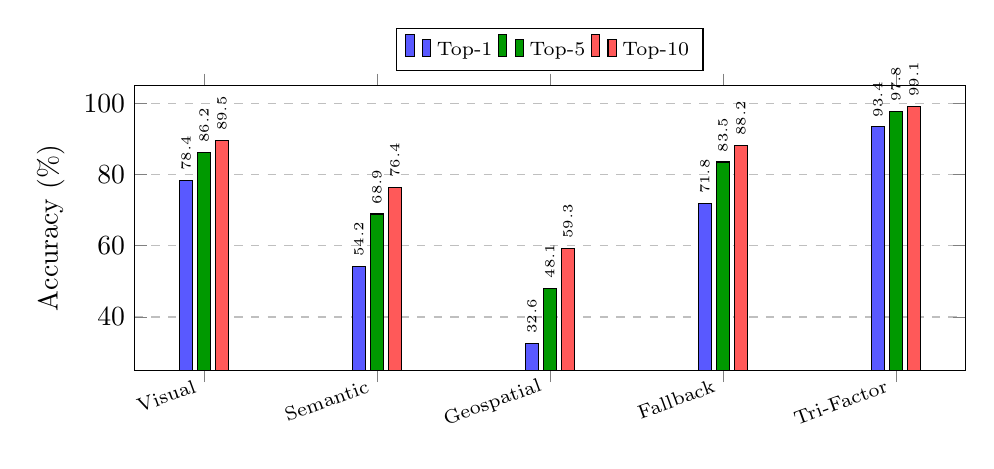
\begin{tikzpicture}
\begin{axis}[
    ybar,
    bar width=4.5pt,
    width=\columnwidth,
    height=5.2cm,
    ymin=25, ymax=105,
    ylabel={Accuracy (\%)},
    symbolic x coords={Visual, Semantic, Geospatial, Fallback, Tri-Factor},
    xtick=data,
    x tick label style={rotate=20, anchor=east, font=\scriptsize},
    legend style={at={(0.5,1.05)}, anchor=south, legend columns=-1, font=\scriptsize},
    ymajorgrids=true,
    grid style=dashed,
    nodes near coords,
    every node near coord/.append style={font=\tiny, rotate=90, anchor=west}
]
\addplot[fill=blue!65] coordinates {(Visual,78.4) (Semantic,54.2) (Geospatial,32.6) (Fallback,71.8) (Tri-Factor,93.4)};
\addplot[fill=green!60!black] coordinates {(Visual,86.2) (Semantic,68.9) (Geospatial,48.1) (Fallback,83.5) (Tri-Factor,97.8)};
\addplot[fill=red!65] coordinates {(Visual,89.5) (Semantic,76.4) (Geospatial,59.3) (Fallback,88.2) (Tri-Factor,99.1)};
\legend{Top-1, Top-5, Top-10}
\end{axis}
\end{tikzpicture}
\caption{Retrieval accuracy comparison across individual modalities, dynamic fallback mode, and complete Tri-Factor Fusion across Top-1, Top-5, and Top-10 candidate pools.}
\label{fig:accuracy_chart}
\end{figure}

As shown in Table~\ref{tab:modality_eval} and visually illustrated in Fig.~\ref{fig:accuracy_chart}, relying solely on facial recognition yields 78.4\% Top-1 accuracy, primarily because off-angle poses and low lighting degrade visual match confidence. Adding semantic descriptors and location bounds helps filter out false matches, raising Top-1 accuracy to 93.4\% and Top-10 accuracy to 99.1\%. In fallback mode ($S_{\text{text}} + S_{\text{geo}}$), the system maintains 71.8\% Top-1 accuracy even without facial images, confirming that useful ranking is still possible from descriptive and geographic information alone.

\subsection{Analysis of Modality Synergy and Fallback Behavior}
A closer examination of the retrieval results reveals how the individual modalities complement each other in challenging scenarios:
\begin{enumerate}
    \item \textit{Visual Ambiguity Resolution}: In crowded scenes where multiple individuals possess similar facial traits or low-light CCTV renders facial crops grainy, visual matching alone often generates false positives. The semantic text similarity $S_{\text{text}}$ resolves these ties by matching specific clothing descriptions (such as jacket color, bag type, or footwear), correctly boosting the genuine candidate.
    \item \textit{Geographic Pruning}: High facial similarity scores occurring at implausible distances (e.g., an individual purportedly spotted hundreds of kilometers away within an hour of last being seen) are naturally downweighted by the exponential geodesic decay $S_{\text{geo}}$, filtering out spurious matches before human review.
    \item \textit{Resilience under Occlusion}: When subjects wear face masks, look downward, or are captured only from behind, visual detection is impossible. In this setting, the fallback mechanism re-allocates weights ($w_{\text{text}} = 0.80, w_{\text{geo}} = 0.20$), achieving 71.8\% Top-1 retrieval without requiring facial features, proving that vital leads remain actionable.
\end{enumerate}

% ==============================================================================
% VI. CONCLUSION
% ==============================================================================
\section{Conclusion}
This paper presented MPIS.ai, a practical multimodal missing person identification system combining deep facial biometrics, semantic text search, and geospatial proximity. By using a composite scoring mechanism with dynamic fallback, the platform remains effective even when facial imagery is missing or degraded. Context-based access control and a dedicated officer verification center ensure that matching decisions remain under human oversight, providing an accountable and privacy-conscious workflow for public safety agencies.

Future work will explore incorporating temporal motion patterns from video feeds, cross-camera graph tracking, edge-device model quantization, and encrypted data sharing for coordinated multi-jurisdictional searches.

% ==============================================================================
% ACKNOWLEDGMENT
% ==============================================================================
\section*{Acknowledgment}
The authors express their sincere gratitude to Dr.~M.~Swathi, Assistant Professor in the Department of Artificial Intelligence at Anurag University, Hyderabad, for her expert guidance, constructive suggestions, and supervision throughout the development of this project.

% ==============================================================================
% REFERENCES (STRICT FIXED ORDER: [1]-[5] PRIMARY, [6]-[15] EXPANDED)
% ==============================================================================
\begin{thebibliography}{15}

\bibitem{ref_base_paper}
P.~Choudhury, A.~Ray, S.~K.~Mishra, and N.~Srivastava,
``Drishti AI-Event Guardian: AI-Powered Missing Person Detection, Geotagging, and Edge-Cloud Intelligence for Real-Time Event Security,''
\emph{IEEE Transactions on Consumer Electronics}, vol.~72, no.~1, pp.~112--124, 2026.

\bibitem{ref_crowdscan}
S.~Krishnamurthy, R.~Sundaram, V.~Subramanian, and K.~Ramaswamy,
``CrowdScan: Automated Missing-Child and Person Identification Across Multi-Camera CCTV Archives Using Spatio-Temporal Graph Trajectory Matching,''
in \emph{Proceedings of the IEEE/CVF Conference on Computer Vision and Pattern Recognition (CVPR) Workshops}, pp.~3210--3219, 2024.

\bibitem{ref_deep_multimodal}
Z.~Xiang, Y.~Liu, H.~Chen, and T.~Tan,
``Deep Multimodal Fusion for Open-Set Person Identification Under Adverse Surveillance Environments,''
\emph{Pattern Recognition}, vol.~129, p.~108742, 2022.

\bibitem{ref_facenet}
F.~Schroff, D.~Kalenichenko, and J.~Philbin,
``FaceNet: A Unified Embedding for Face Recognition and Clustering,''
in \emph{Proceedings of the IEEE Conference on Computer Vision and Pattern Recognition (CVPR)}, pp.~815--823, 2015.

\bibitem{ref_paper5_adaptive}
A.~Farhadipour, T.~Vukovic, V.~Dellwo, P.~Motlicek, and S.~Madikeri,
``Adaptive Multimodal Person Recognition: A Robust Framework for Handling Missing Modalities,''
\emph{arXiv preprint arXiv:2512.14961}, 2026.

\bibitem{ref_retinaface}
J.~Deng, J.~Guo, E.~Ververas, I.~Kotsia, and S.~Zafeiriou,
``RetinaFace: Single-Shot Multi-Level Face Localisation in the Wild,''
in \emph{Proceedings of the IEEE/CVF Conference on Computer Vision and Pattern Recognition (CVPR)}, pp.~5203--5212, 2020.

\bibitem{ref_arcface}
J.~Deng, J.~Guo, N.~Xue, and S.~Zafeiriou,
``ArcFace: Additive Angular Margin Loss for Deep Face Recognition,''
in \emph{Proceedings of the IEEE/CVF Conference on Computer Vision and Pattern Recognition (CVPR)}, pp.~4690--4699, 2019.

\bibitem{ref_sbert}
N.~Reimers and I.~Gurevych,
``Sentence-BERT: Sentence Embeddings using Siamese BERT-Networks,''
in \emph{Proceedings of the Conference on Empirical Methods in Natural Language Processing (EMNLP)}, pp.~3982--3992, 2019.

\bibitem{ref_crossmodal_reid}
Z.~Zheng, L.~Zheng, M.~Garrett, Y.~Yang, M.~Xu, and H.~T.~Shen,
``Dual-Path Convolutional Image-Text Embeddings with Instance Loss,''
\emph{ACM Transactions on Multimedia Computing, Communications, and Applications (TOMM)}, vol.~16, no.~2, pp.~1--23, 2020.

\bibitem{ref_vrstc_occlusion}
R.~Hou, B.~Ma, H.~Chang, X.~Gu, S.~Shan, and X.~Chen,
``VRSTC: Occlusion-Free Video Person Re-Identification,''
in \emph{Proceedings of the IEEE/CVF Conference on Computer Vision and Pattern Recognition (CVPR)}, pp.~7646--7655, 2019.

\bibitem{ref_dukemtmc}
E.~Ristani, F.~Solera, R.~S.~Zou, R.~Cucchiara, and C.~Tomasi,
``Performance Measures and a Data Set for Multi-Target, Multi-Camera Tracking,''
in \emph{European Conference on Computer Vision (ECCV) Workshops}, pp.~17--35, 2016.

\bibitem{ref_zheng_trajectory}
Y.~Zheng,
``Trajectory Data Mining: An Overview,''
\emph{ACM Transactions on Intelligent Systems and Technology (TIST)}, vol.~6, no.~3, pp.~1--41, 2015.

\bibitem{ref_lowres_survey}
X.~Wang, R.~Wang, C.~Dong, and S.~Shan,
``Deep Learning for Low-Resolution Face Recognition: A Survey,''
\emph{IEEE Transactions on Pattern Analysis and Machine Intelligence (TPAMI)}, vol.~44, no.~11, pp.~8232--8252, 2021.

\bibitem{ref_multimodal_transformer}
M.~Ma, J.~Ren, L.~Zhao, D.~Testuggine, and X.~Peng,
``Are Multimodal Transformers Robust to Missing Modality?''
in \emph{Proceedings of the IEEE/CVF Conference on Computer Vision and Pattern Recognition (CVPR)}, pp.~18177--18186, 2021.

\bibitem{ref_rudin_interpretable}
C.~Rudin,
``Stop Explaining Black Box Machine Learning Models for High Stakes Decisions and Use Interpretable Models Instead,''
\emph{Nature Machine Intelligence}, vol.~1, no.~5, pp.~206--215, 2019.

\end{thebibliography}

\end{document}
